% Generated by build_report.py; shared presentation content.
\section{Kiến trúc mô hình BR-Dummy: các bước xử lý}
Mục tiêu: tìm địa điểm quan tâm (\textbf{POI}, như trạm sạc hoặc bệnh viện) mà không gửi GPS thật. Đọc sơ đồ theo \textbf{1 $\to$ 2 $\to$ 3a/3b $\to$ 4 $\to$ máy chủ $\to$ 5}; khung xanh là mô hình.

\begin{center}
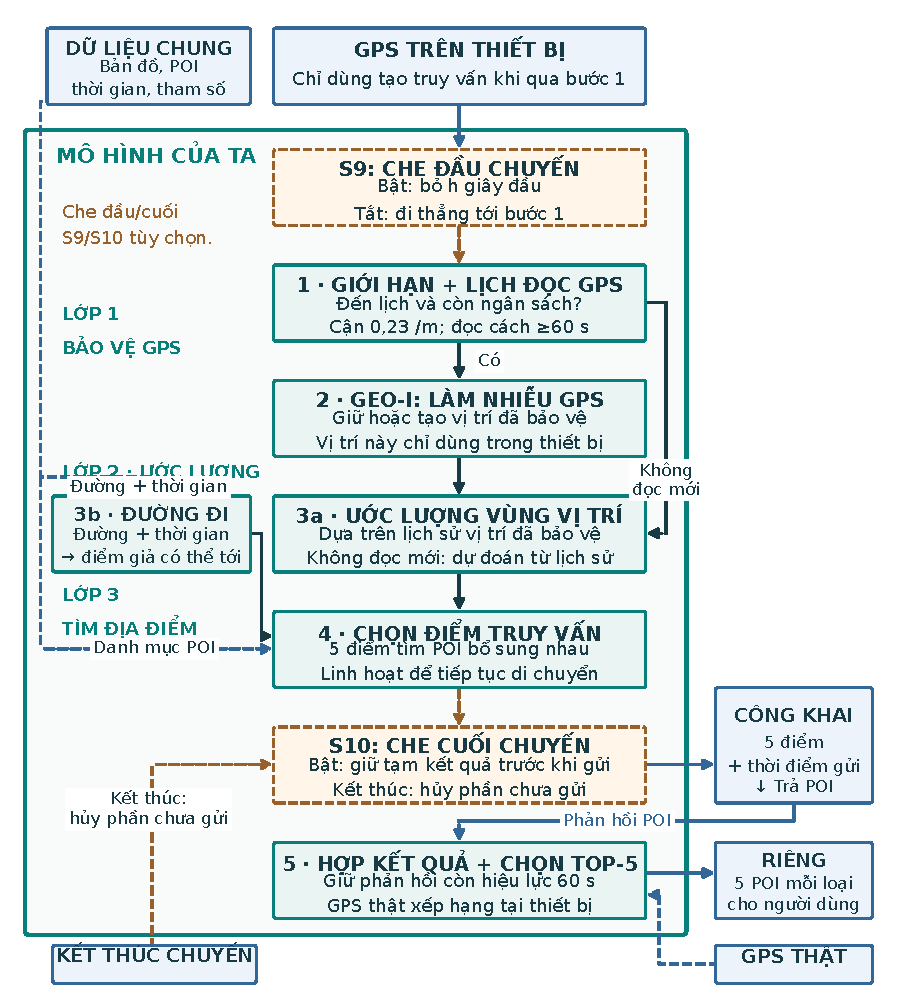
\includegraphics[width=\linewidth,height=0.79\textheight,keepaspectratio]{figures/architecture_report_flow.pdf}
\end{center}
Chưa đến lịch hoặc hết ngân sách thì bỏ bước 2, dùng lịch sử đã bảo vệ. Hai bước 3a/3b cùng giúp chọn điểm truy vấn. Bước 5 nhận kết quả từ máy chủ. S9/S10 là phần mở rộng tùy chọn để che đầu/cuối chuyến.


\clearpage
\subsection{Mỗi bước làm gì và vì sao cần?}
\textbf{Vị trí đã bảo vệ} là tọa độ tham chiếu đã làm nhiễu bằng Geo-I, chỉ dùng trong thiết bị. Từ đó mô hình chọn \textbf{điểm truy vấn giả (dummy)} để gửi thay GPS thật.

\begingroup\small
\begin{longtable}{@{}P{5.006cm}P{11.913cm}@{}}
\toprule
\textbf{Bước / scenario} & \textbf{Cách hoạt động và mục đích}\\\midrule
\endfirsthead
\toprule
\textbf{Bước / scenario} & \textbf{Cách hoạt động và mục đích}\\\midrule
\endhead
\bottomrule\endfoot
1. Giới hạn + lịch đọc GPS — S2/S3 & Kiểm tra lịch đọc và ngân sách còn lại. Không đọc GPS mới để chọn truy vấn khi chưa đến lịch hoặc không đủ ngân sách.\\
\addlinespace[3pt]
2. Geo-I: làm nhiễu GPS — S1/S2 & Phép kiểm tra có nhiễu quyết định giữ vị trí tham chiếu cũ hoặc tạo vị trí mới. Tái dùng giảm các mẫu nhiễu mới khi quan sát lặp.\\
\addlinespace[3pt]
3a. Ước lượng vùng vị trí (belief) & Dùng lịch sử vị trí đã bảo vệ để ước lượng người dùng có thể ở đâu; không coi một tọa độ nhiễu là vị trí chính xác.\\
\addlinespace[3pt]
3b. Kiểm tra đường đi — S3 & Từ điểm giả trước đó, hướng làn, luật rẽ và thời gian, xác định các điểm tiếp theo xe có thể tới.\\
\addlinespace[3pt]
4. Chọn điểm truy vấn — dịch vụ & Chọn 5 điểm có thể trả về các POI bổ sung nhau. Ưu tiên điểm giúp tiếp tục di chuyển tới vùng có kết quả hữu ích.\\
\addlinespace[3pt]
5. Hợp kết quả + chọn top-5 & Giữ phản hồi còn hiệu lực trong 60 giây; hợp các POI nhận được. GPS thật chỉ xếp hạng trên thiết bị để chọn 5 POI mỗi loại.\\
\addlinespace[3pt]
Che đầu chuyến — S9 & Khi bật: không đưa GPS của h giây đầu vào các bước tạo điểm truy vấn.\\
\addlinespace[3pt]
Che cuối chuyến — S10 & Khi bật: giữ tạm kết quả trước khi gửi. Khi chuyến kết thúc, hủy phần chưa gửi để không công bố đoạn cuối.\\
\end{longtable}
\endgroup
Các bước 3–4 chỉ dùng vị trí đã bảo vệ, bản đồ và POI công khai. Có 5 điểm giả không tự bảo đảm ẩn danh. Hai cơ chế che đầu/cuối đã kiểm tra tích hợp, chưa benchmark kết hợp với dịch vụ.

\subsection{Định lượng hai cấu hình Geo-I}
\textbf{GeoI-Paced:} bản so sánh nội bộ. \textbf{GeoI-Slack:} thêm độ linh hoạt khi chọn điểm truy vấn. Hai bản dùng cùng ngân sách riêng tư và cùng dịch vụ. Ngân sách là cận lý thuyết cho cả phiên, không phải tỷ lệ attacker đoán đúng.

\begingroup\small
\begin{longtable}{@{}P{3.938cm}P{6.350cm}P{6.350cm}@{}}
\toprule
\textbf{Tham số} & \textbf{GeoI-Paced} & \textbf{GeoI-Slack}\\\midrule
\endfirsthead
\toprule
\textbf{Tham số} & \textbf{GeoI-Paced} & \textbf{GeoI-Slack}\\\midrule
\endhead
\bottomrule\endfoot
Geo-I / ngân sách & $\varepsilon$\_\allowbreak{}test = $\varepsilon$\_\allowbreak{}release = 0,01 /m; θ = 200 m; cận phiên 0,23 /m & Giống GeoI-Paced\\
\addlinespace[3pt]
Lịch đọc / giữ kết quả & Dùng GPS mới để tạo truy vấn cách $\ge$60 giây; giữ phản hồi còn hiệu lực trong khoảng 60 giây & Giống GeoI-Paced\\
\addlinespace[3pt]
Dịch vụ & K=5 điểm truy vấn; máy chủ trả L=10 POI/loại/điểm; thiết bị chọn 5 POI mỗi loại & Giống GeoI-Paced\\
\addlinespace[3pt]
Độ linh hoạt (slack) & Chọn điểm theo mức phủ POI hiện tại & Cho phép giảm tối đa 0,03 điểm đánh giá độ phủ để đi tới vùng hữu ích hơn; không phải giảm Recall 3\%\\
\end{longtable}
\endgroup
\key{Đóng góp: phối hợp lịch sử vị trí đã làm nhiễu, lịch đọc và ngân sách, đường xe đi được và chất lượng tìm POI. Geo-I + điểm giả đã có tiền lệ [\href{https://wrap.warwick.ac.uk/id/eprint/183198/1/WRAP-privacy-preserving-querying-mechanism-high-utility-electric-vehicles-2024.pdf}{R12}]; lợi ích của cách phối hợp cần kiểm tra bằng benchmark.}

